% !TEX encoding = UTF-8 Unicode

\documentclass[a4paper]{article}

\usepackage{color}
\usepackage{url}
\usepackage[T2A]{fontenc}
\usepackage[utf8]{inputenc}
\usepackage{graphicx}

% -------- Za prikazivanje koda -----
\usepackage{listings}

\definecolor{dkgreen}{rgb}{0,0.6,0}
\definecolor{gray}{rgb}{0.5,0.5,0.5}
\definecolor{mauve}{rgb}{0.58,0,0.82}

\lstset{frame=tb,
  language=C,
  aboveskip=3mm,
  belowskip=3mm,
  showstringspaces=false,
  columns=flexible,
  basicstyle={\small\ttfamily},
  numbers=none,
  numberstyle=\tiny\color{gray},
  keywordstyle=\color{blue},
  commentstyle=\color{dkgreen},
  stringstyle=\color{mauve},
  breaklines=true,
  breakatwhitespace=true,
  tabsize=3
}
% -----------------------------

\usepackage[english,serbian]{babel}

\usepackage[unicode]{hyperref}
\hypersetup{colorlinks,citecolor=green,filecolor=green,linkcolor=blue,urlcolor=blue}

\begin{document}

\title{Napadi na softverske sisteme i mehanizmi zaštite\\ \small{Seminarski rad u okviru kursa\\Metodologija stručnog i naučnog rada\\ Matematički fakultet}}

\author{Čedomir Dimić, Jana Milutinović, Miloš Samardžija\\ dimiccedomir@gmail.com, jana\_milutinovic@yahoo.com, mi13304@alas.matf.bg.ac.rs}

\maketitle
\begin{abstract}
U ovom radu su ukratko objašnjena tri najvažnija aspekta sigurnosti softvera, prikazani su najčešći napadi na softverske sisteme i načini prevencije, greške prilikom dizajna sistema, kao i neki od mehanizama za njihovo otklanjanje i generalno za zaštitu sistema. Specijalno, posvećena je pažnja i bezbednosti Veb servera i propustima koji se javljaju pri implementaciji Veb servera. 
\end{abstract}

\tableofcontents

\newpage


\section{Uvod}
\label{sec:Uvod}

Bezbednost sistema je jedna od najsloženijih tema u modernom     
računarstvu. Povrede bezbednosti snose ogromne posledice najčešće u vidu novca. Stoga, veoma važan zadatak organizacije je da dobro zaštiti poverljive informacije kako one ne bi bile ukradene ili zloupotrebljene.
Sigurnost softvera obuhvata razvoj i implementaciju softvera tako da se on zaštiti od zlonamernih napada i drugih bezbednosnih rizika, ali da istovremeno može da nastavi neometano da radi i pored tih rizika pritom zadržavajući sve predviđene funkcionalnosti. U prethodnom periodu došlo je da značajnog porasta opasnosti i rizika po softverske sisteme, ali i proizvođači softvera ulažu sve veće napore kako bi njihov softver bio što otporniji na moguće napade \cite{softwaresecurity}.


\subsection{Poverljivost, integritet, raspoloživost}
\label{subsec:CIA model}

Kao tri najvažnija aspekta sigurnosti softvera se smatraju poverljivost, integritet i raspoloživost podataka. Ovaj model se često naziva CIA model (eng.~{\em confidentiality, integrity and availability}) \cite{cia}. 

Poverljivost je bliska privatnosti. Mere koje se preduzimaju da bi se obezedila poverljivost su napravljene tako da se onemogući da se osetljive informacije nađu u pogrešnim rukama. Uobičajeno da se podaci klasifikuju u odnosu na to kolika šteta i kakav tip štete je moguć ako oni dođu u neovlašćen posed \cite{cia}.

Integritet uključuje održavanje konzistentnosti, preciznosti i pouzdanosti podataka tokom njihovog čitavog životnog ciklusa. Potrebno je obezbediti da se podaci ne mogu promeniti tokom slanja i da ih ne mogu promeniti ljudi koji za to nemaju ovlašćenje. Kontrola verzija može da služi kao preventiva od pogrešnih promena ili slučajnih brisanja od strane autorizovanih korisnika. Rezervne kopije ili duplikati moraju postojati da bi se podaci koji su oštećeni mogli vratiti u korektno stanje \cite{cia}.

Raspoloživost se postiže održavanjem hardvera, preduzimanjem potrebnih popravki hardvera odmah kada za tim postoji potreba i održavanjem korektnog funkcionisanja operativnog sistema. Takođe je potrebno redovno vršiti ažuriranja sistema. Da bi se izbeglo da podaci postanu neraspoloživi potrebno je da postoje rezervne kopije podataka na geografski izolovanim lokacijama osiguranim čak i od prirodnih nepogoda kao što su požari, poplave i ostale prirodne nepogode. Dodatna oprema kao što je zaštitni zid (eng.~{\em firewall}) se može koristiti da bi se onemogućilo da podaci postanu neraspoloživi zbog zlonamernih napada kao što su onemogućavanje usluga (eng.~{\em denial-of-service}) i upadi u mrežu \cite{cia}. 


\section{Mehanizmi zaštite softverskih sistema}
\label{sec:mehanizmi zastite softverskih sistema}

Da ne bi došlo do narušavanja bezbednosti softvera on mora imati odgovarajuće mehanizme začtite. Neki od osnovnih mehanizama zaštite na Internetu su: \textbf{zaštitni zid} (eng.~{\em firewall}), \textbf{antivirusni programi} koji sprečavaju da na računar dospe zlonamerni softver (eng.~{\em malware}) ili ga uklanjaju po dospeću na računar, \textbf{šifrovanje podataka} i \textbf{virtuelna privatna mreža}.   

\subsection{Zaštitni zid}
\label{subsec:zastitni zid}

Zaštitni zid je mrežni sistem zaštite koji se koristi za praćenje i kontrolisanje dolazećeg i odlazećeg mrežnog saobraćaja. Zaštitni zid uglavnom funkcioniše tako što uspostavlja barijeru između sigurne untrašnje mreže i druge, spoljašnje mreže, kao što je npr. Internet za koji se pretpostavlja da nije siguran.
Zaštitni zid postoji u mrežnoj i desktop varijanti. Mrežni zaštitni zidovi omogućavaju zaštitu cele mreže i svih računara u njoj. Mogu biti softverski koji se izvršavaju na hardveru opšte namene ili hardverski zasnovani.
Zaštitni zid zasnovan na desktop varijanti predstavja sloj softvera na jednom računaru koji kontroliše dolazeći i odlazeći mrežni saobraćaj isključivo na jednom računaru \cite{firewalls}.

\subsection{Antivirusni softver}
\label{subsec:antivirusni softver}

Antivirusni softver je računarski softver koji se koristi da zaštiti, otkrije i ukloni zlonamerni softver sa računara.
Antivirusni program se sastoji od nekoliko programa koji pokušavaju pronaći, sprečiti i ukloniti viruse i ostali zlonamerni softver. Obično koristi dve tehnike da bi postigao svoju funkcionalnost: skeniranje fajlova tražeći poznate viruse proverom definicija u rečniku virusa i identifikacija sumnjivog ponašanja računarskog programa, koje bi mogle biti posledica infekcije. Što se tiče prve tehnike, problem je u tome što se vrlo često pojavljuju novi virusi i čak i pored redovnog ažuriranja postoje novi virusi koje antivirus nema registrovane u svojoj bazi podataka \cite{antivirus}.

\subsection{Šifrovanje podataka}
\label{subsec:sifrovanje podataka}

Zbog mogućnosti da neko zlonameran neovlašćeno prati komunikaciju koja se odvija preko Interneta i to kasnije zloupotrebi, u savremenom poslovanju mora postojati mehanizam koji obezbeđuje:  zaštitu tajnosti informacija (sprečavanje otkrivanja njihovog sadržaja),  integritet informacija (sprečavanje neovlašćene izmene informacija) i autentičnost informacija (definisanje i proveru identiteta pošiljaoca). Kriptografija kao nauka koja se bavi metodama očuvanja tajnosti informacija pruža rešenje ovog problema. Poruke se šifrovanjem transformišu iz čitljivog u nečitljiv oblik za korisnika kome tekst nije namenjen. Samo korisnik kome je tekst namenjen može putem dešifrovanja videti njegov sadržaj.

Asimetrično šifrovanje ili šifrovanje javnim ključem je šifarski sistem u kome svaki učesnik koristi dva ključa – javni i privatni. Javni se može slobodno distribuirati putem elektronske pošte ili Veb sajta, dok je drugi privatni, i dostupan je samo njegovom vlasniku. Moguće je bilo kome poslati šifrovanu poruku, ako je poznat javni ključ osobe kojoj se šalje, a samo primalac svojim privatnim ključem može da dešifruje poruku \cite{cryptography}.

\subsection{Virtuelna privatna mreža}
\label{subsec:virtuelna privatna mreza}

Virtuelna privatna mreža (eng.~{\em Virtual private network}) je virtualizovano proširenje privatne mreže putem javne mreže kao što je Internet. Ona omogućava korisnicima da šalju i primaju podatke preko deljene ili javne mreže stvarajući utisak kao da su njihovi uređaji direktno povezani preko privatne mreže. Aplikacije koje rade preko virtuelne privatne mreže zato mogu biti funkcionalnije i sigurnije nego privatna mreža. Virtuelna privatna mreža obezbeđuje poverljivost tako da čak i da je sadržaj na mreži ukraden na paketskom nivou, napadač će videti samo enkriptovane podatke. Takođe, postoji autentikacija pošiljaoca da bi se neovlašćenim korisnicima onemogućio pristup
mreži \cite{firewalls}.

\section{Napadi}
\label{sec:napadi}
Programeri se uglavnom fokusiraju na korektnost softvera, odnosno na postizanje željenog ponašanja softvera. Bezbednost se odnosi na sprečavanje neželjenog ponašanja. Razmatraju se problemi u dizajnu i implementaciji, koji bi potencijalno mogli da učine aplikaciju ranjivom i neotpornom na napade hakera koji aktivno pokušavaju da zaobiđu bezbednosne mere, i iskoriste i najmanju slabost koju pronađu. Mnogi proboji bezbednosnih mera nastaju upravo zbog ranjivosti softvera. Defekti u softveru se javljaju kada se softver ne ponaša korektno, odnosno kada ne uspeva da zadovolji sve zahteve.

Zbog izuzetno velike složenosti softvera, pojava bagova (eng.~{\em bug}) je neminovna. Normalni korisnici nikad ne primete većinu bagova. Većina bagova koji se jave nakon puštanja softvera u rad se otkrije sasvim slučajno, i uglavnom su posledica neobrađivanja graničnih slučajeva. Bilo bi neisplativo da se svi bagovi pronađu i otklone pre puštanja u rad. Zbog toga se uglavnom ispravljaju samo bagovi za koje je velika verovatnoća da će na njih naleteti normalni korisnici. Pod terminom 'normalni korisnici' se podrazumevaju korisnici koji će softver koristiti na standardan način, za obavljanje posla za koji je softver namenjen, i neće pokušavati da ga iskoriste u druge svrhe za koje nije namenjen, pronalaženjem propusta na koje se ne može naići normalnom upotrebom. Hakeri nisu normalni korisnici. Za normalnog korisnika, slučajno pronalaženje baga će rezultovati nasilnim zatvaranjem programa (eng.~{\em crash}). Hakeri će aktivno raditi na pronalaženju bagova, kako bi ih kasnije iskoristili u svoje svrhe \cite{softwaresecurity}.

Da bismo obezbedili softver, potrebno je eliminisati sve bagove i propuste u dizajnu, ili barem otežati ili u potpunosti onemogućiti njihovo iskorišćavanje \cite{top10flaws}. Otežavanje iskorišćavanja propusta umesto njihovog rešavanja treba razmotriti isključivo ukoliko njihovo rešavanje zahteva velike izmene koje zahtevaju određeno vreme. Čak i tada, to treba da bude samo privremeno rešenje.

Neki od najučestalijih napada su prekoračenje bafera (eng.~{\em buffer overflow}), podmetanje SQL upita (eng.~{\em SQL injection}), zloupotrebljavanje kolačića (eng.~{\em cookies}) i skrivenih polja u različite svrhe, krađa sesije, CSRF i XSS \cite{frontmatter}.
Preduslov za navedene napade je nedovoljna validacija i obrada korisničkog unosa, kao i nepažnja i nestručnost korisnika.

\subsection{Prekoračenje bafera}
\label{subsec:bufferoverflow}
Prekoračenje bafera je bag koji pogađa programe pisane na programskom jeziku nižeg nivoa (eng.~{\em low-level programming language}), uglavnom C i C++, i uvodi značajnije bezbednosne propuste. Do problema dolazi kada program pokuša da upiše količinu podataka koja je veća od veličine bafera. Pisanjem izvan granica bafera se može izazvati oštećenje podataka, nasilno zatvaranje programa ili izvršavanje zlonamernog koda. Mnoge funkcije koje manipulišu memorijom ne vrše proveru da li je došlo do prekoračenja granica nekog bafera, i na taj način se lako može prebrisati vrednost preostalih promenljivih na steku (eng.~{\em stack}) \cite{smashingthestack}.

Fragment koda ~\ref{lst:buffoverflow} prikazuje kako se na jednostavan način može uticati na bezbednost. U ovom primeru, u bafer veličine 4 je upisana niska dimenzije 8, i na taj način je prebrisala vrednost promenljive koja predstavlja indikator da li je korisnik autentikovan ili nije. U tabeli ~\ref{tab:stack} se nalazi stanje steka nakon poziva funkcije strcpy.
\begin{lstlisting}[title={Primer prekoračenja bafera},label={lst:buffoverflow}]
void func(char *arg1)
{
	int authenticated = 0;
	char buffer[4];
	strcpy(buffer, arg1);
	if(authenticated) { ...
}

int main()
{
	char *mystr = "AuthMe!";
	func(mystr);
	...
}
\end{lstlisting}


%\begin{figure}[h!]
%\begin{center}
%\includegraphics[scale=0.75]{slike/stack.jpeg}
%\end{center}
%\caption{Stanje steka nakon izvršavanja strcpy}
%\label{fig:stack}
%\end{figure}

\begin{table}[h!]
\begin{center}
\caption{Stanje steka nakon izvršavanja strcpy}
\begin{tabular}{|c|c|c|c|c|c|c|c|}
 \multicolumn{8}{c}{}\\
 \multicolumn{1}{c}{} & \multicolumn{1}{c}{m} & \multicolumn{1}{c}{e} & \multicolumn{1}{c}{!} & \multicolumn{1}{c}{\textbackslash0} & \multicolumn{3}{c}{}\\ \hline
A u t h & 4d & 65 & 21 & 00 & \textcolor{blue}{\%ebp} & \textcolor{blue}{\%eip} & \&arg1\\ \hline
 \multicolumn{1}{c}{buffer} & \multicolumn{4}{c}{authenticated} & \multicolumn{3}{c}{}\\
\end{tabular}
\label{tab:stack}
\end{center}
\end{table}

Navedeni primer je bio samo jedan od načina kako se ovaj bag može iskoristiti u korist napadača. Umesto proizvoljne promenljive na steku, napadač je mogao da izmeni adresu povratka iz funkcije, i na taj način može da izvrši proizvoljni zlonamerni kod. Pored ovog napada, postoje i varijacije poput prekoračenja hipa (eng.~{\em heap overflow}), prekoračenja celog broja (eng.~{\em integer overflow}), prekoračenje čitanjem (eng.~{\em read overflow}), itd.

\subsection{Podmetanje SQL upita}
\label{subsec:sqlinjection}
Podmetanje SQL upita omogućava izvršavanje zlonamernih SQL upita. Ovo je jedan od najstarijih, najčešćih i najopasnijih napada na Veb aplikacije. Ranjiva je svaka aplikacija koja koristi bazu podataka, i pritom ne vrši validaciju korisničkog unosa. Iskorišćavanjem propusta, u određenim okolnostima, napadač može da zaobiđe mehanizme autentikacije i autorizacije, i da pročita sadržaj baze podataka. Takođe, može da dodaje, modifikuje i briše zapise, čime direktno utiče na integritet podataka, a potencijalno i na dostupnost aplikacije.

Da bi izveo napad, napadač prvo mora da pronađe tačke u aplikaciji koje zahtevaju korisnički unos, a da pritom ti uneseni podaci učestvuju u nekom SQL upitu koji je ranjiv. Upiti su ranjivi ukoliko se korisnički unos direktno uključuje u upit, bez prethodne validacije i pretprocesiranja \cite{sqlinjection1}.

Primer ~\ref{lst:sqlinjectionex1} prikazuje ranjivost u slučaju kada podaci nisu prethodno validirani. Ukoliko se za vrednost promenljive \emph{passwd} postavi \textbf{' OR 1=1}, nakon zamene se dobija upit prikazan na ~\ref{lst:sqlinjectionex2}. Izvršavanjem ovog upita, iz tabele \emph{users} će biti izlistani svi korisnici.
\begin{lstlisting}[title={Primer ranjivog upita},label={lst:sqlinjectionex1}]
uname = request.POST['username']
passwd = request.POST['password']

sql = "SELECT id FROM users WHERE username='" + uname + "' AND password='" + passwd + "'"

database.execute(sql)
\end{lstlisting}
\begin{lstlisting}[title={Upit nakon zamene sa vrednošću promenljivih},label={lst:sqlinjectionex2}]
-- uname = "username"
-- passwd = "' OR 1=1"
SELECT id FROM users WHERE username='username' AND password='' OR 1=1;
\end{lstlisting}

Jedan od načina za odbranu od ovakvih napada je upotreba pripremljenih i parametrizovanih upita (eng.~{\em prepared statements}). Kod ovog pristupa, SQL upiti se parsiraju od strane servera baze podataka nezavisno od bilo kakvih parametara.

\subsection{Krađa sesije}
\label{subsec:sessionhijacking}
Krađa sesije (eng.~{\em session hijacking}) jedan je od načina zloupotrebe kolačića. Usled nedostatka stanja u HTTP protokolu, za identifikaciju sesije u Veb aplikacijama se koriste kolačići, tzv. identifikatori sesije. Ukoliko napadač na neki način dođe u posed ovog kolačića, može ga iskoristiti tako što će se predstaviti kao neki drugi korisnik, i izvršavaće akcije u njegovo ime. Na taj način zaobilazi mehanizme autentikacije i autorizacije, i može da utiče na poverljivost i integritet podataka.

Preduslov za ovaj napad je nestručnost i nepažnja korisnika, kao i da sesija nije istekla. Neki od načina kojima može da dođe u posed identifikatora sesije je instalacija zlonamernih dodataka za Veb pregledač koji imaju pristup svim kolačićima, uključujući i one skrivene, ili nadgledanjem mreže, ukoliko aplikacija koristi nebezbednu vezu.

Sprečavanje ovakvih napada se vrši korišćenjem skrivenih kolačića, instalacijom dodataka isključivo iz proverenih izvora i korišćenjem bezbedne veze. Ukoliko bilo šta od navedenog izostane, korisnik je izložen ovom napadu.

\subsection{CSRF}
\label{subsec:csrf}
CSRF (eng.~{\em cross-site request forgery}) je napad koji krajnjem korisniku nameće da izvrši neželjene akcije nad Veb aplikacijom u kojoj je trenutno autentikovan. Mete ovog napada su zahtevi koji vrše izmenu stanja, ali napadaču to ne omogućava da ukrade podatke, jer ne postoji način da vidi odgovor na ove zahteve. Uz malu pomoć socijalnog inžinjeringa (eng.~{\em social engineering}) (slanjem linkova putem e-maila ili ćaskanja (eng.~{\em chat}), napadač može da prevari korisnika neke Veb aplikacije izvršavanjem neželjenih akcija. Ako je žrtva normalan korisnik, uspešan CSRF napad može nametnuti korisniku da izvrši zahtev koji menja stanje (npr. vrši transfer novca, menja e-mail adresu). Ali ukoliko je žrtva neki administrativni nalog, napad može ugroziti celu aplikaciju \cite{csrf1}. Razlog zašto ovaj napad uspeva je to što zlonamerna osoba ne mora da bude autentikovana da bi izvršila prevaru, već prevarene korisnike navodi da sami izvrše nepoželjnu akciju.

Napad se može sprečiti upotrebom csrf tokena. Ideja je da se token generiše na početku sesije, i da se uključi u svaki zahtev, tako da server može da ga iskoristi u proveri legitimnosti zahteva. Da bi napadač zaobišao ovaj mehanizam, morao bi da pogodi token, a to je praktično nemoguće, zbog same složenosti tokena.

\subsection{XSS}
\label{subsec:xss}
XSS (eng.~{\em cross-site scripting}) je napad zasnovan na umetanju koda koja napadaču omogućava da izvrši zlonamerni JavaScript u drugom Veb pregledaču. Napadač ne cilja direktno njegovu žrtvu, već iskorišćava propuste u aplikaciji koju žrtva posećuje, kako bi kasnije preuzela zlonamerni kod. Gledano iz perspektive pregledača, zlonamerni JavaScript predstavlja legitiman deo sajta. Jedini način koji napadaču omogućava da izvrši zlonamerni kod je da ga umetne direktno u jednu od stranica koje žrtva posećuje. To je moguće ukoliko se korisnički unos direktno uključuje kao sastavni deo stranice, bez validacije, zato što napadač može da unese tekst koji će biti tretiran kao kod od strane JavaScript interpretera.

XSS napadi se dele na:
\begin{itemize}
\item \textbf{postojani XSS} (eng.~{\em persistent XSS}), gde maliciozni kod potiče iz baze podataka
\item \textbf{reflektovani XSS} (eng.~{\em reflected XSS}), gde maliciozni kod potiče iz zahteva žrtve (npr. URL)
\item \textbf{DOM-zasnovani XSS} (eng.~{\em DOM-based XSS}), gde je ranjivost na klijentskoj strani
\end{itemize}

Napad se sprečava enkodiranjem korisničkog unosa, tako da ga pregledač interpretira isključivo kao podatke. Ipak, u nekim slučajevima samo enkodiranje podataka nije dovoljno da bi se odbranilo od napada. To su slučajevi gde se korisnički unos direktno umeće u \textit{<script>} tagove, u atribute za rukovaoce događajima (event handlers), ili u CSS. Jedan od načina da se ovo spreči je da se jednostavno izbegava umetanje korisničkog unosa na takva mesta. Neki od veb pregledača implementiraju određene mehanizme odbrane od XSS napada koristeći statičku analizu (npr. Chrome Anti-XSS Filter).

\section{Uobičajene greške u dizajnu softvera}
\label{sec:uobicajene greske u dizajnu softvera}

Iako sistem uvek može da ima grešaka u implementaciji ili bagova, siugurnost mnogih sistema je narušena zbog propusta u dizajnu \cite{top10flaws}.
Neke od njih su:
\begin{itemize}
\item \textbf{Nikada ne treba imati previše poverenja.}
    Dizajn gde se autorizacija, kontrola pristupa, sprovođenje bezbednosnih mehanizama ili osetljivi podaci nalaze na klijentskom softveru misleći da tu neće biti otkriveni ili promenjeni od strane veštih korisnika ili zlonamernih hakera je suštinski slab. Treba biti siguran da su svi podaci koji su primljeni od nepouzdanog klijenta validirani pre obrade.
\item \textbf{Treba koristiti mehanizam autentikacije koji ne može da se zaobiđe.}
    Autentikacija predstavlja potvrđivanje identiteta subjekta. Cilj sigurnog dizajna je da spreči subjekta (korisnika, napadača) da pristupi sistemu ili servisu bez prethodne autentikacije. Kada se koristnik autentikuje, sistem bi trebalo da takođe spreči korisnika da promeni svoj identitet bez ponovne autentikacije.
\item \textbf{Autorizacija posle autentikacije.}
    Iako je važno da se izvrši autentikacija identiteta korisnika pre nego što im se omogući da koriste sistem ili da izvode određene akcije, to može i da ne bude dovoljno pre nego što se odluči da li je moguće korisniku dozvoliti da izvodi određene akcije. Autorizacija treba da predstavlja eksiplicitnu proveru i neophodna je i posle inicijalne autentikacije. Autorizacija ne zavisi samo od privilegije koje neki korisnik ima, nego i od konteksta određenog zahteva.
\item \textbf{Precizno odvojiti podatke od kontrolnih instrukcija i nikada ne obrađivati instrukcije primljene od nepouzdanih izvora.}
    Nedostatak odvajanja podataka od koda često dovodi do nepouzdanog toka izvršavanja softverskog sistema.
\item \textbf{Treba definisati pristup koji osigurava da su svi podaci eksplicitno validirani.} 
    Softverski sistemi i komponente često prave pretpostavke o podacima nad kojima rade. Ranjivosti softvera često nastanu zbog implicitnih pretpostavki o podacima koje mogu biti iskorišćene od strane napadača. 
\item \textbf{Koristiti kriptografiju pravilno.} 
    Kriptografija je jedan od najvažnijih alata kojij se koristi za građenje sigurnog sistema. Pravilnim korišcenjem kriptografije može se osigurati poverljivost podataka, mogu se zaštititi podaci od neovlašćenog menjanja itd. S druge strane kriptografija je vrlo teška za implementaciju i tu se može javiti dosta propusta.
\item \textbf{Identifikovati osetljive podatke i načine rukovanja njima.}
    Jedan od najvažnijih zadataka dizajnera sistema je da identifikuju osetljive podatke i donesu odluke kako da ih pravilno zaštite. Ako dizajneri ne mogu da identifikuju osetljive podatke ili načine na koje ti podaci mogu da budu iskorišceni onda sistem neće pravilno zaštititi te podatke.
\item \textbf{Uvek obratiti pažnju na korisnike.}
    Način na koji korisnik interaguje sa sofverom zavisi ne samo od dizajna i implementacionih odluka dizajnera nego i od kongitivnih sposobnosti korisnika. Kao posledica toga, dizajneri i arhitekte bi trebalo da uzmu u obzir i fizičke sposobnosti, kulturološke predrasude, navike i sklonosti korisnika sistema i načine na koji te osobine korisnika mogu uticati na ukupunu sigurnost sistema.
\item \textbf{Treba razumeti kako eksterne komponente utiču na mogućnost napada na sistem.}
    Kad se dodaju funkcionalnosti postojećem sistemu, razvijaoci često koriste postojeće komponente da bi dodali neke ili sve nove funkcionalnosti. Treba biti siguran da je softver koji se dodaje testiran i da zadovoljava sigurnosne standarde u postojećem softveru. Trebalo bi obratiti pažnju na to da uključivanjem eksternih komponenti uključujemo i sve njihove sigurnosne nedostatke i ograničenja.
\item \textbf{Treba biti fleksibilan kad se uzimaju u obzir buduće promene na subjektima i objektima.}
    Sigurnost softvera mora biti dizajnirana tako da može da se menja, a ne da bude krhka i statična. Softver, okruženje u kome se pokreće softver i opasnosti se menjaju tokom vremena i prilikom dizajniranja softvera potrebno je voditi računa i mogućim promenama u budućnosti.
\end{itemize}

\section{Bezbednost i Veb serveri}
\label{sec:bezbednosni propusti prilikom implementacije Veb servera}

Veb server (eng.~{\em Web Server}) je računar koji je odgovoran za preuzimanje i opsluživanje Veb stranica koje zahteva klijent. Veb server obrađuje klijentske zahteve preko HTTP mrežnog protokola čiji je zadatak da distribuira informacije na Internetu. On je povezan na Internet što znači da korisnici mogu da pristupe podacima sa servera sa bilo kog mesta na Internetu. Ovakva vrsta javnog pristupa može imati za posledicu pokušaje neovlašćenog pristupa podacima od strane hakera, radi onesposobljavanja nekih servisa ili krađe vrednih podataka. Postoji veliki broj tipova Veb servera od kojih su najpoznatiji Apache Web Server, Internet Information Server (IIS) , lighttpd , Sun Java System Web Server i Jigsaw Server. \\
\indent Veb serveri su najčešće mete napada na mreži. Zbog toga je važno da se zaštite na odgovarajući način, kako bi eventualna zloupotreba imala što manje posledica. Zaštita servera je zahtevtevan i tehnički izazovan posao koji obuhvata uočavanje potencijalnih mesta i načina napada, kao  i implementaciju mehanizama zaštite istih.  

\subsection{Bezbednosni propusti i načini otklanjanja}
\label{sec:propusti}
Kao što je pomenuto, serveri su najizazovnije mete napada od strane hakera, koji iskorišćavaju različite bezbednosne mane infrastrukture servera radi kompromitovanja sistema. U najčešće bezbednosne pretnje po Veb server se ubrajaju: \textbf{neovlašćeni pristup}, \textbf{nepravilna upotreba}, \textbf{onemogućavanje usluga (eng.~{\em Denial of service}} i \textbf{fizičke pretnje}. Zaštita servera obuhvata odbranu "u dubinu", građenjem sloj po sloj različitih zaštitnih mehanizama u okviru arhitekture mreže, operativnog sistema i aplikativnog sloja  \cite{wssg}. Zaštita u dubinu pruža dobru prevenciju i zaštitu od napada na server.

\indent U prethodnom poglavlju su opisane uobičajene greške u dizajnu softvera i većina njih se odnosi i na Veb servere. Osim njih, neki specifični propusti za Veb servere su:  
\begin{itemize}
    \item \textbf{Bagovi u CGI skriptama }\\
    \textbf({eng.~{\em  Common Gateway Interface (CGI)}}) skripte su programi koji se na Veb serverima izvršavaju u realnom vremenu i čija je uloga da rukuju ulaznim podacima korisnika, pristupaju bazi i vraćaju informacije korisniku \cite{lawsa}. U suštini, to su mini Veb serveri čija je uloga važna, te greške u ovim skriptama mogu dovesti do kompromitovanja servera na dva načina. Prvi je otkrivanjem važnih host informacija koje mogu da pomognu napadačima da pristupe serveru, dok je drugi način kada korisnikki ulazni podaci mogu biti komande koje se automatski izvršavaju i kao takve da nanesu štetu host mašini i ugroze sigurnost servera.
    
    
     \item \textbf{ Kontrola pristupa }  
     
  \textbf{Kontrolom pristupa} regulište se ko ima mogućnost pretraživanja i izvršavanja (CGI skripti) na serveru. Pravilno podešena autentikacija, autorizacija i kontrola pristupa su obavezni kako bi se smanjio broj bezbednosnih povreda. Kontrolom čitanja nekih fajlova se štiti poverljivost informacija a kontrolom
     pristupa se štiti njihov integritet. Obratiti pažnju na dobru zaštitu konfiguracijskih fajlova, čijim bi se pristupom mogla ugroziti sigurnost celog servera. \\
     \indent Pravilno konfigurisana kontrola pristupa smanjuje mogucnost otkrivanja osetljivih informacija koje ne smeju biti javno izložene. Takođe, dobra kontrola pristupa će ograničiti korišćenje resursa u slučaju DoS napada \cite{gspws}. 
     Primarni uređaji za kontrolu pristupa su ruter i zaštitni zid.
     Na slici ~\ref{fig:server} prikazan je jedan ispravan način konfiguracije Veb servera.
    \begin{figure}[h!]
    \begin{center}
    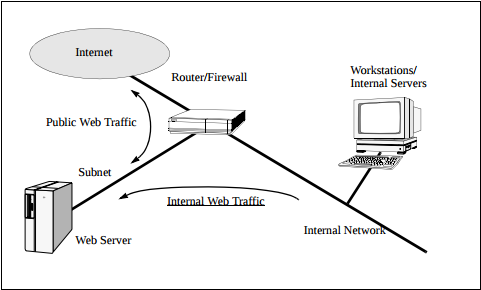
\includegraphics[scale=0.6]{slike/server.png}
    \end{center}
    \caption{Konfiguracija Veb Servera \cite{scpws}}
    \label{fig:server}
    \end{figure}
    \item \textbf {Loša bezbednosna konfiguracija } \\
    Dobra konfiguracija servera je veoma važna i predstavlja osnovu za kvalitetnu zaštitu od napada. Često se pri konfiguraciji neke važne bezbednosne stavke zanemare:
    
    \begin{itemize}
        \item Čuvanje mreže direktorijuma na serveru može prouzrokovati curenje važnih informacija
        \item Korišćenje nestabilnih ili zastarelih verzija softvera
        \item Izvršavanje nepotrebnih servisa na mašini
        \item Menjanje podrazumevanih šifri je obavezno
        \item Otkrivanje informacija o rukovanju greškama (eng.~{\em  stack traces})  
    \end{itemize} 
        
    \item \textbf{ Greške pri autorizaciji } \\
    Na serveru, autorizacija korisnika uvek mora da bude korektno izvršena! U suprotnom, poverljive informacije mogu biti otkrivene i menjane pa je veoma važno zaštititi različite osteljive datoteke tako da im se ne može pristupiti bez autorizacije. 
   
    \item \textbf{Obezbediti mehanizme logovanja} \\
    Logovi su dnevnici u kojima se cuvaju podaci o tome ko je i kada modifikovao, dodavao i pristupao serverskim komponenatama. Posmatranje i analiza log datoteka su neophodni, s obzirom da su oni cesto i jedini pokazatelji sumnjivih aktivnosti. Kako bi logovanje dalo najvise rezultata, poželjno je obezbediti mehanizme alarmiranja, kako bi se administrator što pre obavestio o potencijalnim sumnjivim aktivnostima prepoznatim u logovima. Log datoteke bi trebalo smestiti na određeno mesto tako da ne zauzimaju puno prostora na hard disku. Takođe, važno je praviti i rezervne kopije ( eng.~{\em  backup}) logova kako bi se u slučaju njihovog nestanka ustanovili sumnjivi pristupi. 
  \end{itemize}
  
  U ovom poglavlju opisani su neki najčešći bezbednosni propusti pri implementaciji Veb servera čijim se zanemarivanjem ozbiljno ugrožava njihova sigurnost. Kompleksnost samog Veb servera zahteva jaku bezbednosnu zaštitu, a pored pomenutih koncepata treba obratiti pažnju i na još neke aspekte sigurnosti:
   
   \begin{itemize}      
    \item Obezbediti dobru zaštitu od virusa 
    \item Jako je važno postojanje sistema za prevenciju i prepoznavanje upada 
    \item Implementirati jaku enkripciju lozinki 
    \item Zaštititi server od poznatih i čestih napada
    \item Konfigurisati server tako da se ograniče funkcionalnosti programa, skripti i plug in-ova \cite{scpws}
    \item Problem može biti nedovoljna mrežna bezbednosna kontrola i nesiguran dizajn hostovane aplikacije
      \end{itemize}



\section{Zaključak}
\label{sec:zakljucak}
Potrudili smo se da ukratko prikažemo koji su najčešći napadi na softverske sisteme, na koji način on može biti ugrožen i kako se možemo zaštititi. Može se primetiti da validacija i obrada korisničkog unosa igraju veliku ulogu u sprečavanju velikog broja napada. Međutim, pored svih mehanizama zaštite koji postoje, softver nikada ne može biti u potpunosti bezbedan i potrebno je konstantno pratiti kakve se nove opasnosti po softver pojavljuju i zaštititi se na odgovarajući način. S obzirom na to da je bezbednost softvera veoma kompleksna i široka oblast, u ovom kratkom radu nisu mogli biti obuhvaćeni svi aspekti bezbednosti softvera i mi smo se ograničili na neke najvažnije, ali ovaj rad može predstavljati dobar uvod u detaljnije izučavanje pojedinih aspekata bezbednosti softvera koji su prikazani.

\addcontentsline{toc}{section}{Literatura}
\appendix
\bibliography{seminarski} 
\bibliographystyle{plain}

\end{document}
